%Motivation.

% % % % % % % % % % % % % % % % % % % % % % % % % % % % % % % % % % % %

% \subsection{Cosmic complementarity [TT]}
% PJM: I think this could function as the preamble for this section.
% We already have some mention of other probes in earlier sections,
% so it makes sense to motivate the forecasts in the next two subsections
% with the context being joint analysis. What do you think?

In this section we discuss the future of time delay cosmography and
present an ambitious yet realistic roadmap of how to improve the
measurement in the next decade. In order to construct the roadmap, we
will discuss in detail how to decrease the random uncertainties
(i.e. precision; Section~\ref{ssec:precision}), and what systematic
uncertainties will need to be controlled as the random uncertainties
decrease (i.e. accuracy; Section~\ref{ssec:accuracy}).

Before we lay out the roadmap, however, it is good to pause and
reflect on the broader context, and ask whether this is a worthy
endeavour.  Understanding the nature of dark energy is one of the most
profound questions in all of physics, and it is thus not surprising
that the efforts of many scientists and funding agencies have been
directed towards this goal. Dedicated instruments, telescopes, and
satellites are being built or planned with budgets that range from the
tens of millions of dollars into the billions (Euclid, WFIRST). Given
the steep challenges associated with each technique, most scientist
agree that is important to pursue several independent ones at the same
time (DETF, DESC). First, we do not know which techniques will live up
to their promise and which ones will be stymied by hitherto unknown
systematic effects, when we reduce the random uncertainties by one or
more orders of magnitudes. Second, as discussed in the introduction,
extraordinary claims require extraordinay proof, so it will certainly
require more than one independent measurement to convince the
community that, for example, dark energy is not the cosmological
constant ($w\neq-1$).

Given this context, deciding whether time delay cosmography is worth
pursuing boils down to three simpler questions. The first question is
whether time delays contain valuable information {\it independent} of
other cosmological probes. As detailed in Section~\ref{sec:cospars},
the answer is a resounding yes: gravitational time delays are
virtually independent of the uncertainties affecting the other
established probes of dark energy, and provide valuable complementary
information, chiefly on the Hubble constant, which is commonly
regarding as one of the essential ingredients for interpreting other
datasets such a the cosmic microwave background (Hu, Weinberg, Kim).
We will expand on this topic in the remainder of this section by
showing cosmological forecasts for gravitational time delays by
themselves and in combination with other probes.

The second question is whether it is feasible to achieve an {\it
interesting} level of precision and accuracy in coming years. In this
mindset, {\it interesting} is defined as having total uncertainties
comparable to that of other contemporary probes. This will be
discussed in detail below.

The third and final question is what is the {\it cost} of pursuing
this roadmap, and how does it compare to other probes. Our aim is not
to compute a full cost accounting, which will be almost impossible
considering that each probe involves facilities, observatories,
computing and brainpower, well beyond the boundaries of any individual
project, collaboration, or funding agency. Not to mention that the
marginal cost of adding a technique to an existing program or
facility, is very different from what the cost of building a facility
just for that purpose. For example, the cost of monitoring strongly
lensed quasars in LSST data is much less than building and operating
the LSST. Instead, we will aim to give an approximate sense of the
observational and human resources that will be needed to pursue the
roadmap. Having voted with our feet, we obviously think that the
relatively low {\it cost} and the relatively low risk of time delay
cosmology well justifies adding it to the investment portfolio of a
modern cosmologist. Hopefully the rest of this section will give the
reader enough information to make up their own mind on this matter.


%What's the point? Arent' other probes already doing it? Our place in the
%cosmology ecosystem. Refer back to current constraints from \citet{Suy++13} in
%Section~\ref{sec:cospars}, which show other probes.
%Discuss place relative to other distance indicators
%like Cepheids, BAO, Sne. Linder SL + SNe plots.
%Then complementarity with growth of structure
%probes like weak lensing, clusters etc etc. How important is H0?
%Weinberg et al 2013, Kim et al 2014. Figure 48 from Weinberg?

%Importance of multiple INDEPENDENT measurements for discovery of new
%physics, and to ensure overall accuracy of cosmological parameters.
%Define accuracy. Define precision. Segue. cost


% % % % % % % % % % % % % % % % % % % % % % % % % % % % % % % % % %

\subsection{Precision [PJM]}
\label{ssec:precision}

With considerable observational and data analysis effort, the
feasibility of reaching a {\it precision} of 6-7\% in time delay distance
per lens has been demonstrated. The contributions to this statistical
error budget
from the time delay measurement, mass model, and environment
correction are at present approximately equal, and somewhat larger than
the estimated systematic errors. In this situation it makes sense to
enlarge the sample of lenses, in order to beat down the statistical
uncertainties. We return to the question of how to reduce the residual
systematic errors in the next section.

\citet{C+M09b} made initial Fisher matrix forecasts of the likely
available precision on $H_0$ in large future surveys. They considered
several possible samples, concluding that 100 well-measured systems
(with 5\% distance precision each) should provide sub-percent precision
on the Hubble constant, and provide  dark energy parameter constraints
that are competitive with optimistic forecasts of other ``Stage IV''
cosmological probes. They also note that comparable constraints could be
available from a sample of 4000 time delay lens systems, each with only
photometric redshifts and simple image configuration model constraints
\citep[following][]{Ogu07b}.  Continued investigation of both samples
seems warranted, keeping in mind that the size of such a photometric
sample would be set by the availability of time delays measured at the
$\pm$~several day level.

%%%%%%%%%%%%%%%%%%%%%%%%%%%%%%%%%
\begin{figure*}[!ht]
\centering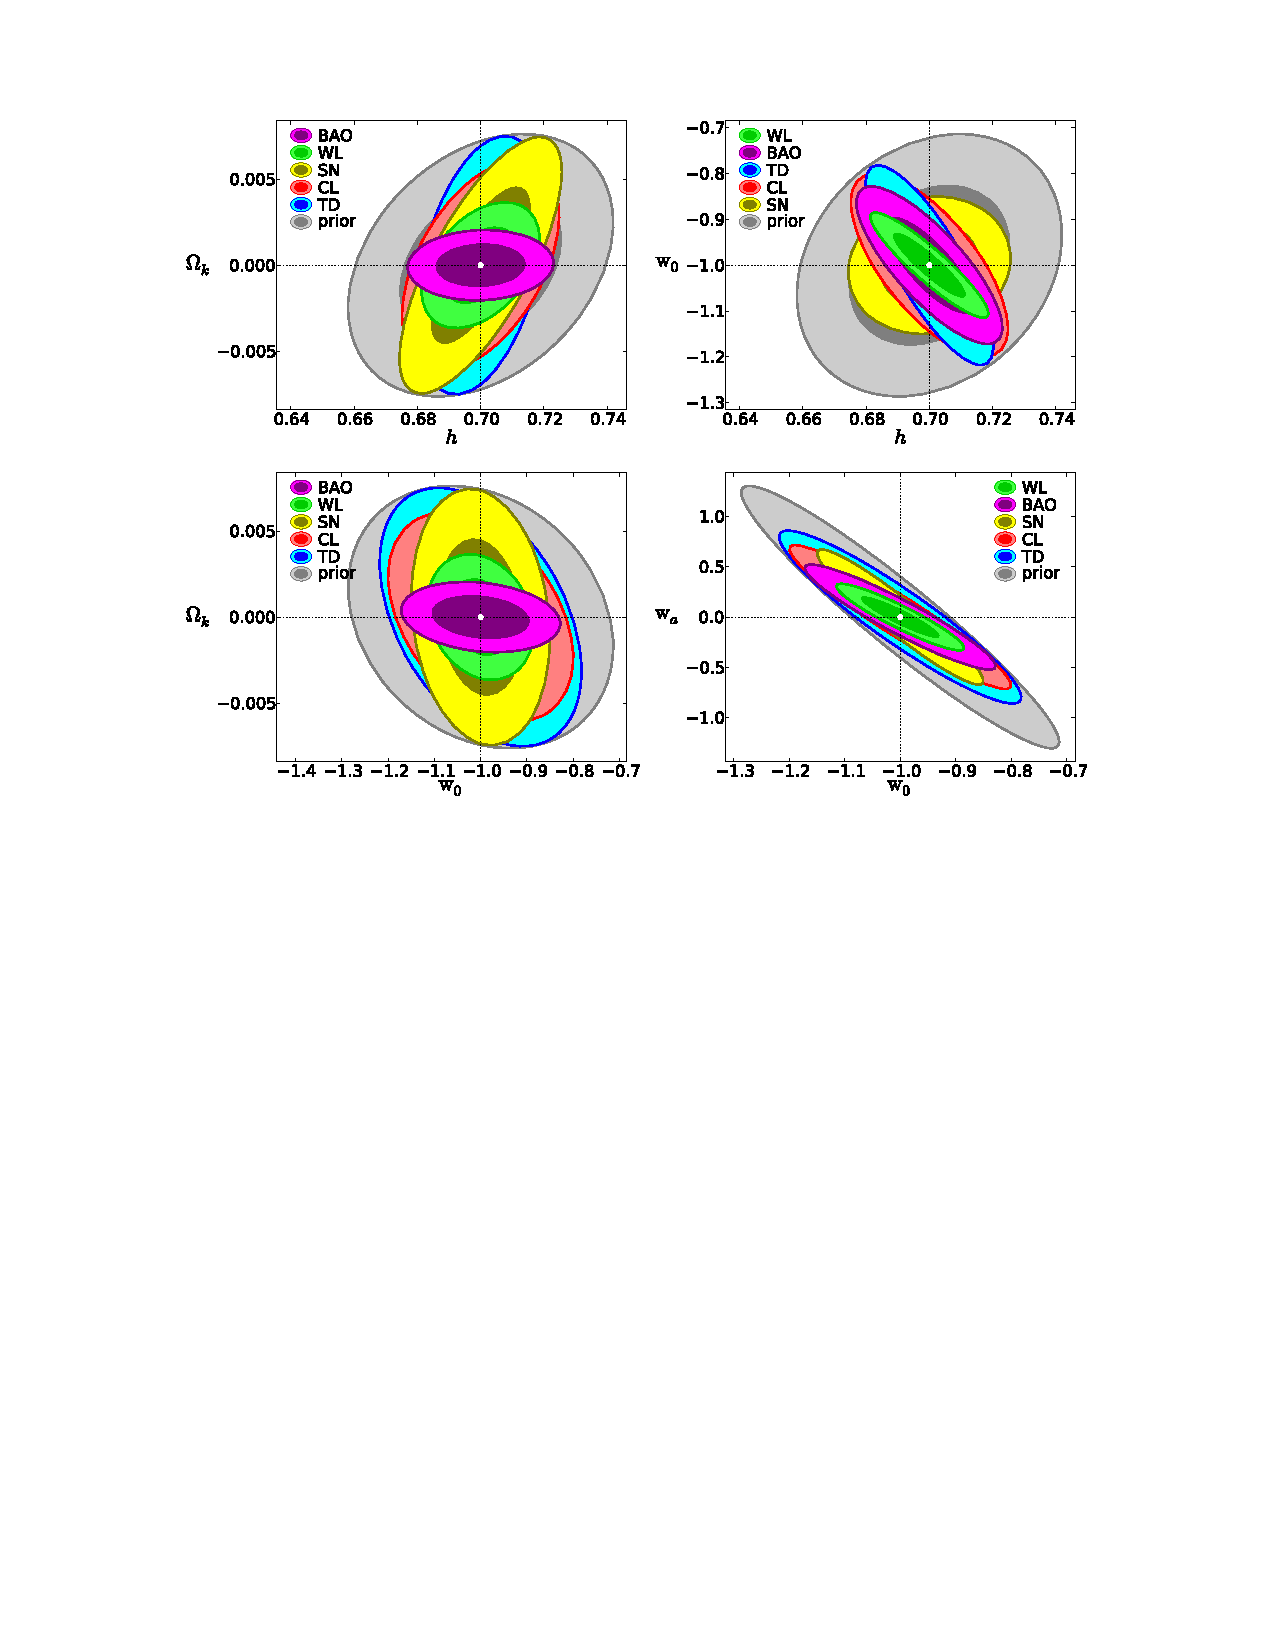
\includegraphics[width=0.9\linewidth]{figures/Coe+Moustakas09_fig14.pdf}
\caption{Fisher matrix forecasts of cosmological parameters, based on
Dark Energy Task Force assumptions and having 5\% distance precision
for each of 100 time delay lenses. The Stage IV cosmological probes
being compared in an  open CDM cosmological model with time-variable
dark energy equation of state are weak lensing (WL), BAO, supernovae
(SN), cluster mass function (CL) and time delay cosmography (TD).
Figure reproduced from \citet{C+M09b}.}
\label{fig:fisher}
\end{figure*}
%%%%%%%%%%%%%%%%%%%%%%%%%%%%%%%%%

% Extrapolations to N lenses assuming X\% precision per time delay
% distance, forecasts.

% FIGURE: Forecasts for 10,50,100,1000 lenses for various cosmological
% models (w, wa+w0, curvature etc etc). CosmoSIS forecasts (ackn. Dave \&
% Elise, ask them).

While Figure~\ref{fig:fisher} allows different cosmological probes to
be compared (and assessed for competitiveness), it does not show the
value of combining those probes. Indeed, \citet{Lin11} found that the
particular combination of a type Ia supernova dataset with a time  delay
lens dataset holds promise, with a sample of 150 time delay distances,
each measured to 5\% precision, improving the dark energy figure of
merit by a factor of about 5 over what could be  plausibly obtained with
a sample of about 1000 Stage 3 supernovae and a Planck CMB prior alone.

More recently, \citet{JeeKomatsuSuyu2015} have pointed out that
cosmological parameter forecasts for time delay lens samples are
conservative, if each lens is assumed only to measure the time delay
distance. Including the angular diameter distance dependence as well can
have a marked effect on the projection, especially if the spectroscopic
constraints on the lens mass distribution are assumed to be very strong.
The reproduction of Figure 5 from
\citet{JeeEtal2016} in the lefthand panel of Figure~\ref{fig:DdDdt}
illustrates this. These authors find that a future sample of
50 lenses
with 5\% measurements of both time delay distance and angular diameter
distance would increase the figure of merit by a factor of two over that
provided by a Stage~3 supernova and BAO joint analysis. The righthand
panel of Figure~\ref{fig:DdDdt} puts such improvements in the  current
observational context. In the B1608$+$656 analysis, the  angular
diameter distance dependence {\it was} accounted for during the
calculation of the predicted time delay and velocity dispersion data,
but the constraints on the angular diameter distance were not strong:
assigning a uniform prior PDF for the cosmological parameters rather
than the distances introduced degeneracy between $\Dd$ and $\Ddt$,
which then seems to have been broken primarily by the time delay
information to yield a $5.7\%$ precision prediction for $\Ddt$, and
a corresponding $8.1\%$ precision prediction for $\Dd$.
With spatially resolved spectroscopy we should anticipate the angular
diameter distance becoming more important in future analyses, with
some work on simulated data needed to quantify this.


%%%%%%%%%%%%%%%%%%%%%%%%%%%%%%%%%
\begin{figure*}[!t]
\begin{minipage}{0.48\linewidth}
    \centering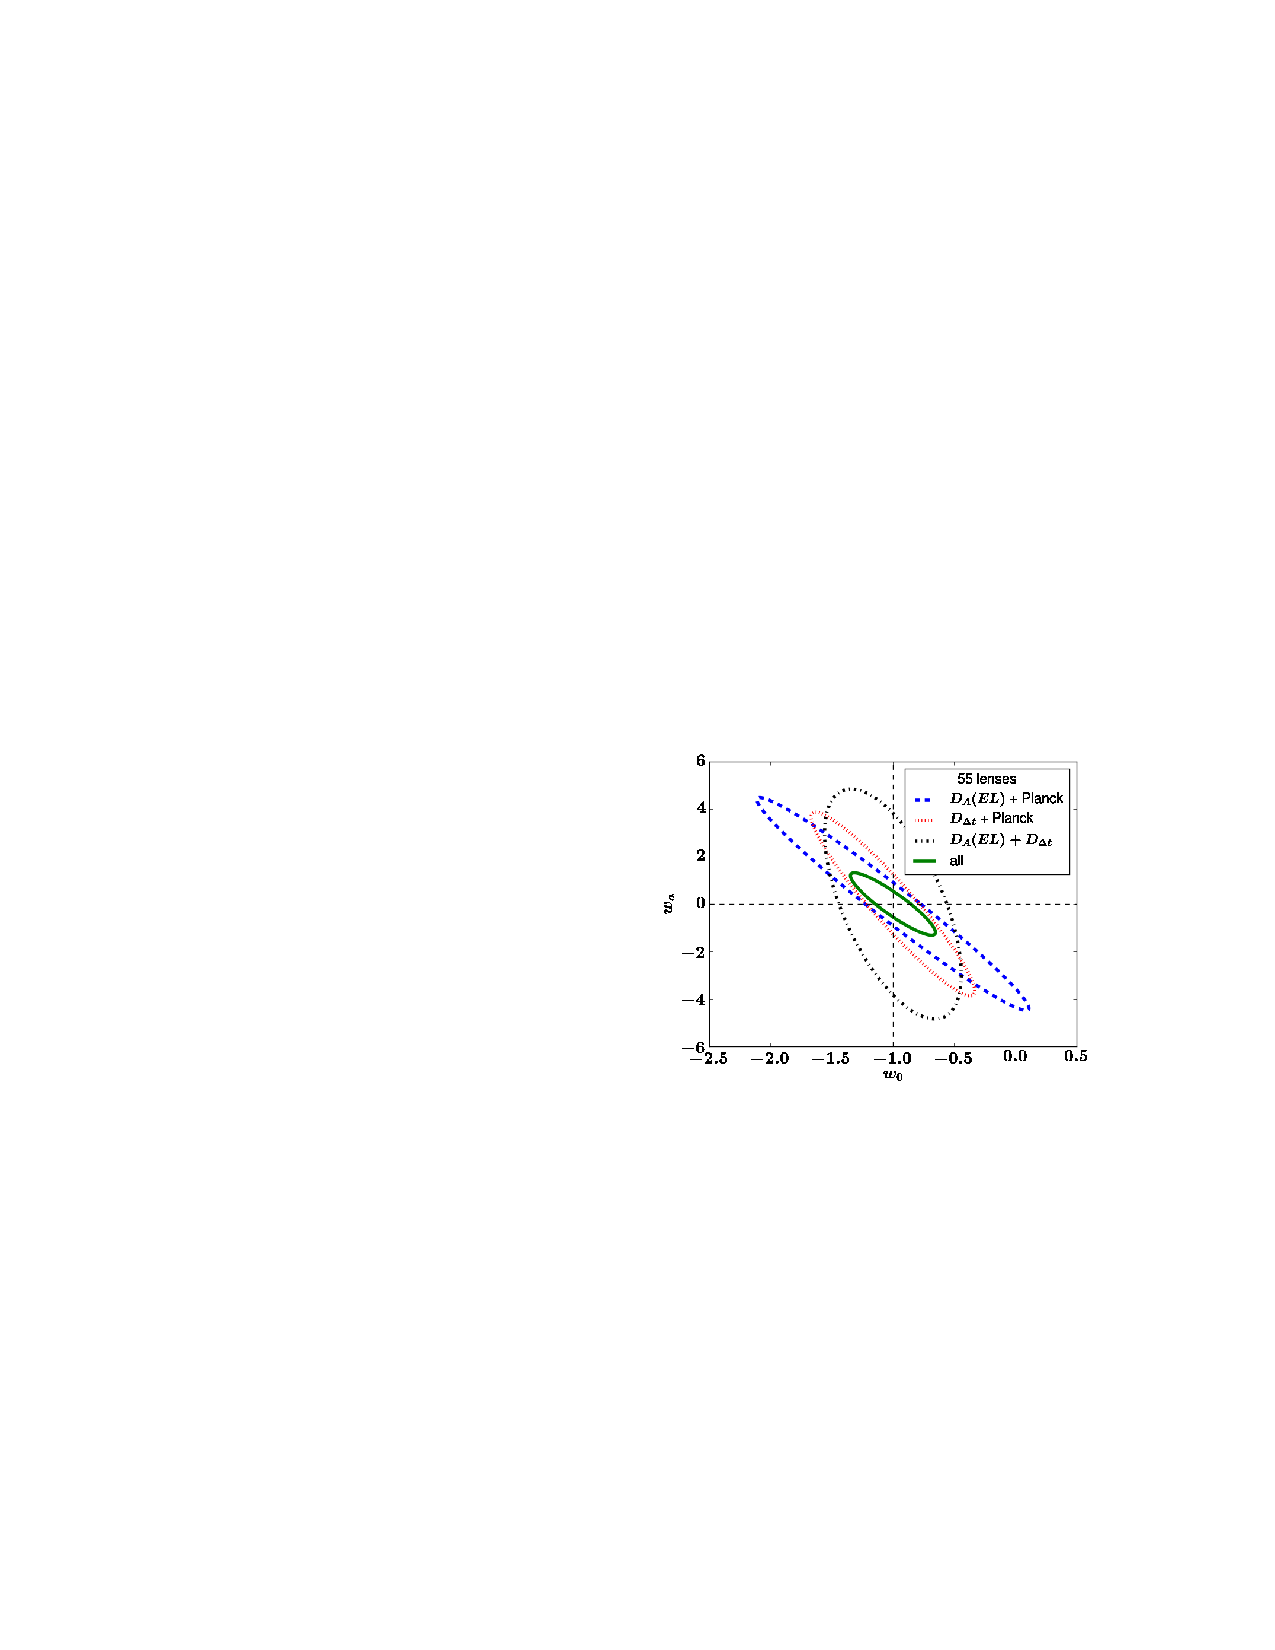
\includegraphics[width=\linewidth]{figures/Jee16_fig5b.pdf}
\end{minipage}\hfill
\begin{minipage}{0.48\linewidth}
    \centering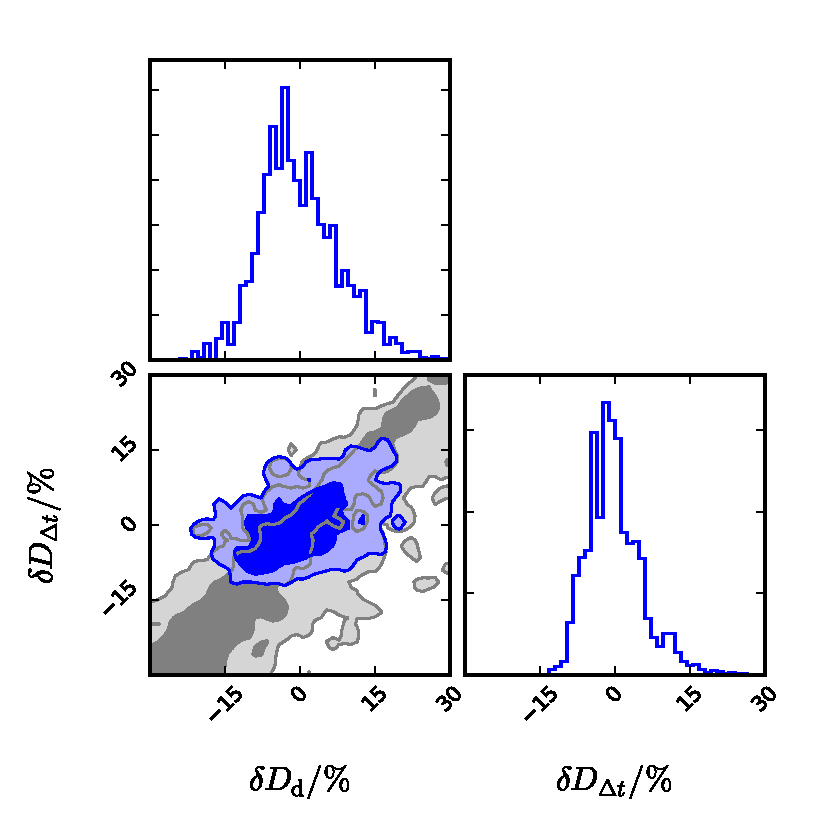
\includegraphics[width=\linewidth]{figures/B1608_DdtDa.pdf}
\end{minipage}
\caption{Cosmological information from angular diameter distances
as well as time delay distances. Left: Fisher matrix
forecasts for a future time delay lens sample where 5\% precision on
each distance is assumed: the combination of distances gives a
significantly more powerful constraint than the time delay distances
would alone \citep[reproduced from][]{JeeEtal2016}. ``$D_{\rm A}(EL)$'' is
the angular diameter distance to the lens from Earth. Right: marginalized
prior (gray) and posterior (blue) PDFs for the two
distances in the B1608$+$656 system, assuming uninformative priors for the
cosmological parameters of a flat $\Lambda$CDM model and offset and
rescaled to reveal the implied percentage precisions of 5.7\% and 8.1\%
in $\Ddt$ and $\Dd$ respectively. }
\label{fig:DdDdt}
\end{figure*}
%%%%%%%%%%%%%%%%%%%%%%%%%%%%%%%%%


What will it take to reach the required level of
distance precision in each of 100 lenses?
If \citet{LiaoEtal2015} are right, samples of over 100 lenses with
precise time delays should be able to be constructed from analysis of
the LSST light curves. The lens models for these systems should be able
to be constrained to sufficient precision using high resolution imaging
from next generation AO facilities, giant segmented mirror telescopes,
JWST and even WFIRST \citep{Men++15}. High overall mass model precision,
and the exploitation of the angular diameter distance dependence,
will require high signal to noise, spatially-resolved spectroscopy as
well: integral field units on
these same telescopes should be able to provide this. The contribution
to the distance uncertainty from the line of sight was particularly high
in the  cases of B1608$+$656 and RXJ1131: in most other systems in a large
sample the effects of the environment should be lesser, and they should
(effectively) average down \citep{Col++13}. The main challenge in
reaching the required Stage IV is likely to be the analysis cost: lens
modeling is something of a craft, and scaling up to large samples could
pose problems. Distributing the work among a large team of modelers will
be needed, an approach that is proving effective in the Frontier Fields
cluster lensing project \citep{FF}.



% % % % % % % % % % % % % % % % % % % % % % % % % % % % % % % % % %

\subsection{Accuracy [PJM]}
\label{ssec:accuracy}

While the precision available from Stage 3 and Stage 4 samples makes
time delay lenses an interesting prospect for cosmology, they will, like
the other probes, be limited by systematic errors. As the forecasts
show, competitive contributions to joint dark energy parameter
inferences correspond to sub-percent distance (or equivalently, Hubble
constant) precision, which implies that the residual systematic error
(that is, post-combination) in  distance needs to be well below 1\% {\it
per lens}. In this section we revisit the primary sources of systematic
error and  assess the prospects for this stringent requirement to be
met.

1) Time delay measurement. Encouragement from TDC1 for single filter
Stage 3 monitoring. How to scale up? Targeted short timescale
monitoring, indications from McCully et al. LSST multi-filter light
curve quality to be checked by TDC2, will hinge on accurate treatment of
color variability and microelensing. Hierarchical approach. AGN physics
as spin-off.

2) Lens mass modeling. Percent-level systematics due to model
assumptions (ie MSD) pointed out by S\&S, investigated in sims by Xu et
al.  IFU observations, resolved stellar kinematics: accuracy challenge.
Flexibilty of mas smodels. UNconstrained pixels replaced by basis sets?
Potential for  informative priors on coefficients, informed by large
numbers of non-lens galaxies.  Assumptions break degeneracies, priors
make this process fuzzy, and somewhat safer. Main piece of information
is self-similarity of massive galaxies:  SL2S work of Sonnenfeld builds
on long FP history to infer scaling  relations in lens galaxies.
Consider ensembles of time delay lenses,  but also all other lenses, to
bring in more information about massive galaxy density structure..

3) Environment and line of sight

Phil is here...

Other things: time delay perturbations (someone's noise is somebody
else's signal..)

The importance of blinding.


% % % % % % % % % % % % % % % % % % % % % % % % % % % % % % % % % %

\subsection{Roadmap [TT]}
\label{ssec:roadmap}

% [DO WE WANT TO HAVE SEPARATE SUBSECTION CALLED ROADMAP, OR IS IT GOING
% TO BE EMBEDDED IN THE TWO SUBSECTIONS ABOVE. I THINK IT MAY BE
% EFFECTIVE TO CALL IT OUT]
